\documentclass{article}
\usepackage[utf8]{inputenc}
\usepackage{mhchem} % símbolos químicos
\usepackage{tabularx}

\usepackage{array} % gestión de tablas
\usepackage{xcolor}
\usepackage{tcolorbox}
\usepackage{graphicx}

\graphicspath{ {img/}}

\title{Unit 3. The Chemical Bond}
\author{Francisco Javier Guijarro}

\begin{document}

	\maketitle

	\section{Introduction. Key Concepts}

		\begin{figure}[htp]
			\centering
			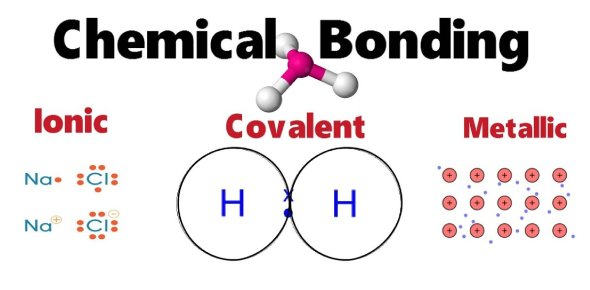
\includegraphics[width=10cm]{chemical_bond_1}
		\end{figure}
	
	
		All chemical elements (except noble gases) combine with each other, 
		because in this manner they are more stable.
		
		\begin{itemize}
				\item A \textbf{chemical bond} is an electrical attraction between atoms. 
				Its purpose it is obtaining a  stable electronic configuration (i.e,  8 electrons in the outer shell (\textbf{valence shell}), except for H and Li that are stable with two electrons in the outer shell.).
				\item \textbf{Valence} or \textbf{valency of an element} is the number of electrons 
				that the element needs or exceeds to have a stable electronic configuration.

		\end{itemize}	
		
		\subsection*{Noble gases}

			They are are called \textbf{inert gases} because they do not combine with any other atom, 
			since they have and already \textbf{stable electronic configuration} in the valence shell.

			Noble gases have \textbf{very low melting and boiling points}.

		\subsection*{Types of chemical bonds}

			\begin{itemize}
				\item \textbf{Covalent bonds}. Characterized by the \textbf{sharing of pairs of electrons} 
				between \textbf{non-metallic atoms}.
				\item \textbf{Ionic bonds}. Characterized by the \textbf{loss of one or more of electrons} 
				in \textbf{metallic atoms}, that are \textbf{gained} by a \textbf{non-metallic} atom.
				\item \textbf{Metallic bonds}. Characterized by the \textbf{sharing or loss pairs of electrons} 
				between \textbf{metallic atoms}.
			\end{itemize}
						
			\begin{center}
				\resizebox{\textwidth}{!}{
					\begin{tabular}{ | m{4cm} | m{4cm} | m{4cm} | m{4cm} | }
						\hline
						\textbf{bond name} & \textbf{covalent} & \textbf{ionic} & \textbf{metallic} \\
						\hline
						\textbf{atoms involved} & non-mettalic & metallic and non-mettalic & mettalic \\
						\hline
						\textbf{description} & sharing pair of electrons & loss of electrons in the metal, 
						that are gained by the non-metal & losing or sharing electrons \\
						\hline
					\end{tabular}
				}
			\end{center}

	\section{The covalent bond}
			Chemical bonding that is characterized by the \textbf{sharing of pairs of electrons} 
			between atoms of \textbf{nonmetals} or \textbf{hydrogens}.

		\subsection{Molecular covalent substances}
			Molecular covalent substances are chemical substances formed by \textbf{molecules}. 
			A \textbf{molecule} is an electrically neutral group atoms held together by 
			\textbf{strong covalent chemical bonds}
			in a \textbf{fixed number}.

			\subsubsection{Molecular formula}
				The molecular formula is the \textbf{symbolic representation} of its molecules. 
				It shows:

				\begin{itemize}
					\item The \textbf{symbols} of the elements.
					\item The \textbf{numerical subscripts}, that indicate the number of atoms of each type. 
				\end{itemize}

				\begin{figure}[htp]
					\centering
					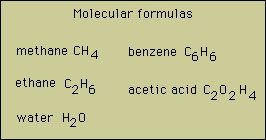
\includegraphics[width=6cm]{formula.jpg}
					\caption{Examples of chemical formulas}
				\end{figure}

			\subsection{Relative molecular mass}
				The relative molecular mass ,\textbf{\textit{$M_{r}$}}, is the mass of one of its molecules.
				It is calculated by adding the atomic masses ,\textbf{\textit{$A_{r}$}},of the atoms taht make up the molecule.

				\[ M_{r}(\ce{H2O}) = 2 \times A_{r}(\ce{H}) + A_{r}(\ce{O}) = 2 \times 1 + 16 = 18\ u\]
			
\end{document}